\documentclass[../main.tex]{subfiles}

\begin{document}

\section{Results}
The results' section presents the findings from the analysis of
the data collected during the simulated intrusion attempts
on the MediColbox.
The data provides insights into the physical movements
and vibrations experienced by the MediColbox during these intrusion scenarios.

\subsection{Analysis of the Data}

The data captured the inertial patterns resulting from different simulated intrusion attempts, including striking, dropping, sawing, and shaking the MediColbox.
The data analysis focused on the accelerometer readings as base point to evaluate the sensitivity and effectiveness of the IMU in detecting unauthorized access. Some of the events will, if relevant, use the gyroscopic data.

\vspace{30px}

\subsubsection{Striking the MediColbox}

This event is an attemp to simulate an intrusion event in the form of
somebody trying to break open the \gls{medicolbox} by hitting the box with something like a hammer that might expose the box to a large force.

Figure \ref{fig:accelerometer_striking} presents the
accelerometer data recorded when the MediColbox was
struck with a fist.

at the start of the graph we can see the reading of the body of the prorotype at rest. it shows an acceleration wit hthe magnitude of approximately $10\;[m/s^2]$ divided among the $z$ and $y$ direction of the sensor. this is the object experiencing the "normal force" which acts upon the object to keep it standing still against the acceleration of gravity. if we are to read $0\;[m/s^2]$ the \gls{imu} will need to be in "free fall". "free fall" is any motion of a body where gravity is the only force acting upon it \cite{Freefall_Encyclopædia_Britannica_2024}. thus, now that we know that the read acceleration is from the normal force, which means it is pointing opposite to the direction of gravity, we can compare the direction of the read acceleratoin with the directions from Figure \ref{fig:xxsensehat_axisinfo} and conclude the orientation of the protoype will be with the face of the \gls{hmi} facing downwards.

When we continue looking at the graph, moving our gaze along the axis of time, the accelerometer readings show a sharp increase in
acceleration, describing the impact during the event of somebody striking the prototype, followed by a swift, and then gradual decrease in acceleration as
the impact of the strike dissipate.
We can see that the acceleration is the same direction as the normal force.
The strike is done from above, striking directly down at the prototype.
The aceleration read is most likely again the normal force, accelerating the prortype back to standing still, resisting the force from the fist.
We should also see the acceleration from the fist hitting the prototype, but it seems the sampling frequency isn't hight enough to pick up all the details in the event.
The peak acceleration value reached during the
strike was measured at
$X = 5\;[m/s^2]$, $Y = -31 [m/s^2]$, $Z = -55\;[m/s^2]$
and occurred at $t = 0.8\;[s]$.
The analysis of the data indicates that the
IMU successfully detected and recorded the impact caused by the
striking event.

\begin{figure}[htbp]
    \centering
    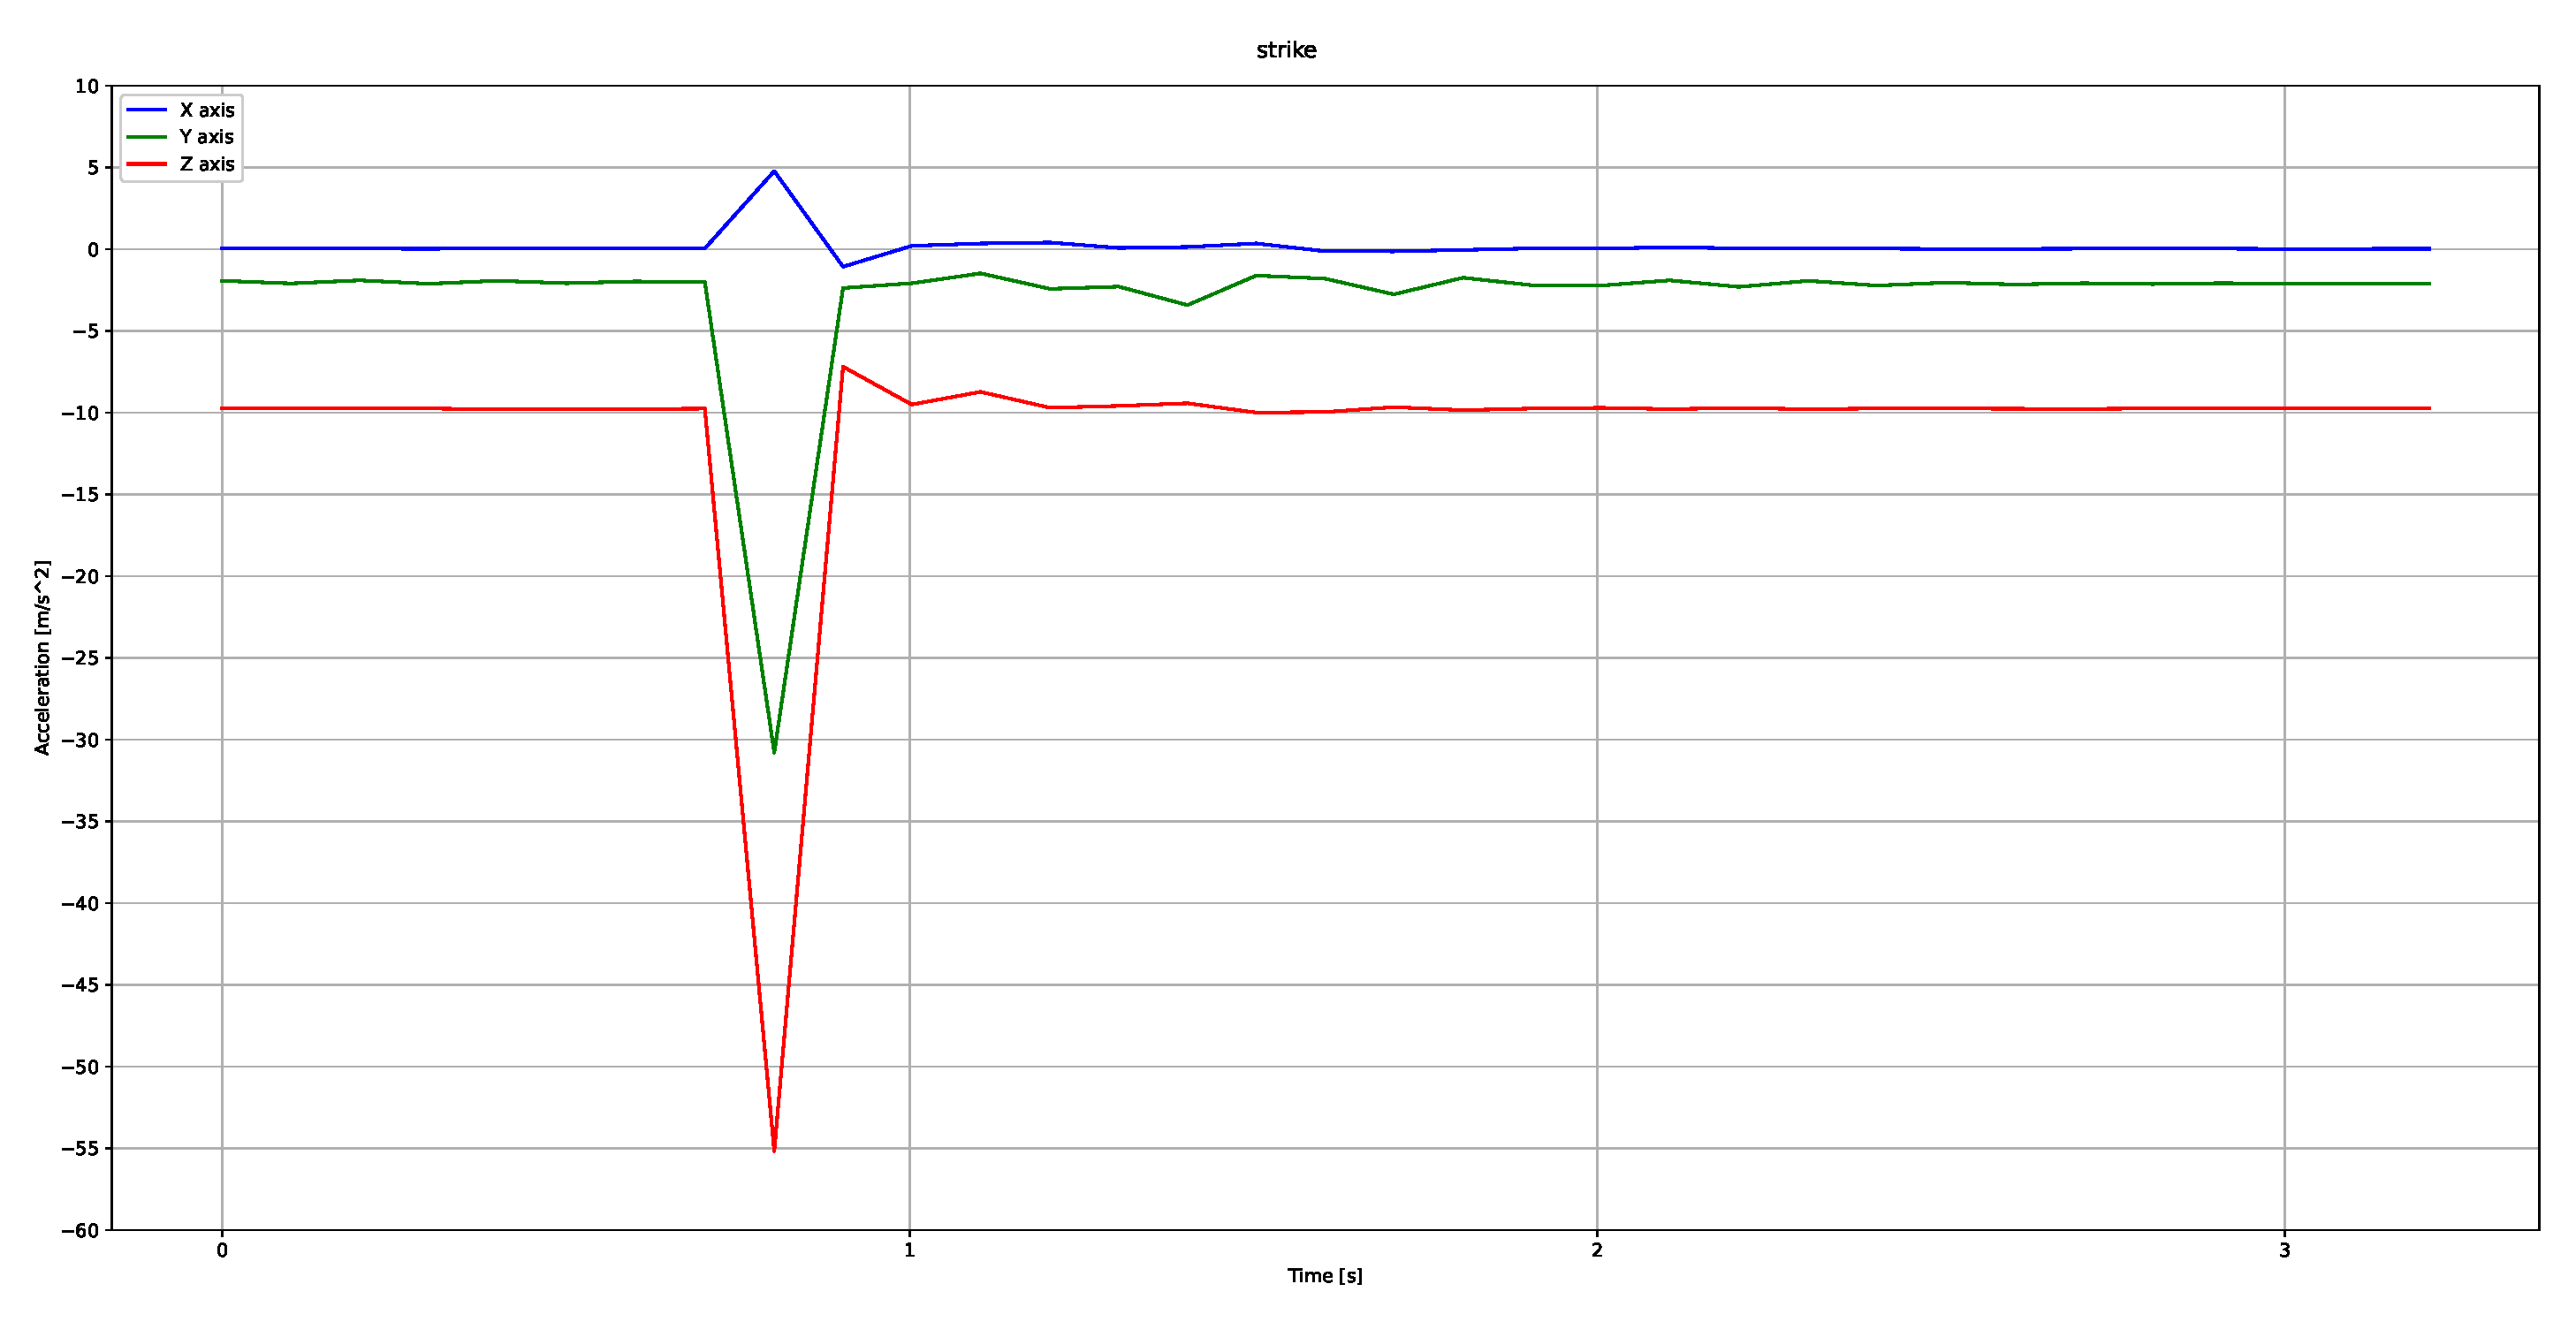
\includegraphics[width=0.8\textwidth]
    {resources/figures/Acceleration_strike.eps}
    \caption{Accelerometer data during the striking event}
    \label{fig:accelerometer_striking}
\end{figure}

Looking at the data we can also see the peak acceleration and how it
stands out from the rest of the data visualized.
However, how do we set criteria so that we can automatically differentiate an attempt of intrusion from just a random event?
A way we, during the data gathering, could reason for, would be to find the force needed to break the box and estimate it from the weight of the box how much acceleration would be close to breaking the box open. In this case the data gathering "Protoype" is $0.645\;[kg]$. With the measured acceleration in $X$, $Y$ and $Z$ direction results in a combined acceleration of $|\overrightarrow{a}| = \sqrt{5^2+(-32)^2+(-55)^2}\;[m/s^2] \approx 63.332\;[m/s^2]$. If a box is designed to handle an impact large enough to momentary expose it to $63.332\,[m/s^2]$ multiplied by a given safety factor, then it would be viable to account for sensor error margins and say that any acceleration above $60\;[m/s^2]$ should immediately trigger an alarm.

If we look back to the begining of this paper, on to how it is mentioned that
the \gls{medicolbox} is tested for impacts up to $8 000\;[N]$, using Newtons second ($F=ma$) law we estimate that a force of $8 000\;[N]$ would be meassured as an acceleration with the magnitude of $93\;[{m/s^2]}$ since it weights $86\;[kg]$. calculating it backwards an acceleration of $60\;[{m/s^2]}$ would result in $5160\;[N]$. That is a massive force, and not something you would just randomly expose an object to without massive effort. To put it in persoective, if you pushed down on a bathroom-weight with the force of $5000\;[N]$ it would show approximately $500\;[kg]$ on the display.
The Prototype is a lot lighter (it only weights $0.645\;[kg]$)
so in reality the impact force is a lot closer to $40\;[N]$ which is a lot less than the $5000\;[N]$ that would be needed to accelerate it similarly. Logically this means that the heavier the box, the lower the criteria will be for meassured acceleration to trigger an alarm, and the more difficult it will be for this method to differentiate an intrusion attempt with random noise.

Another method that could be to assume that if somebody wanted to break the box, they would either break the box in one strike, or try to hit the box repeatedly with strikes that individually might not break the box but that combined might manage to break the bx due to material fatigue. If we divide the strike force that would immediately trigger an alarm (in this case $60\;[m/s^2]$), by the estimated resistance to fatigue in a scale from 0 to 1 and raise it to the number of strikes you assume you would need to break the box using the assumed amount of needed repeated strikes. An example of this could be to do the calculation:

$$a_{Repeated} * {\rho_{fatigue}}^{n_{strikes}} \rightarrow 60 [m/s^2] * 0.9^5 \approx 35.43 [m/s^2] $$

In this example then $5$ repeated strikes of approximately $35.43 [m/s^2]$ will also trigger an alarm.

An algorithm we deviced would be to run two loops, one loop every time we read a value from the IMU.
If the acceleration has a magnitude equal to, or greater than the
strike kriteria $K_{strike}$, then raise the alarm.
additionally, if the acceleration has a magnitude equal to,
or greater than the weaker strike kriteria $K_{repeated}$, increase the value of $n_{repeated}$.
If the value of counted strikes $n_{repeated}$ becomes equal to,
or greater than the criteria of repeated strikes $n_{strikes}$,
which we mentioned in one of the equations earlier, then trigger the alarm.

the second loop will occur periodically with a time interval equalt to $T$, which can be described as:

$$T=\frac{T_{totalCountingTime}}{n_{strikes}}$$

Where $T_{totalCountingTime}$ is the total time span you expect the number of strikes $n_{strikes}$ to happen within.

In the case of striking we have found that $K_{strike} = 60\;[m/s^2]$
combined with $\rho_{fatigue} = 0.9$, $n_{strikes}=5$
and $T_{totalCountingTime}=10\;[s]$
will be optimal values to detect impacts on the prototype.
As the \gls{medicolbox} is substantially heavier,
we will need too lower $K_{strike}$.

% If we continue to analyze the data, we can try using frequency analysis on the striking event hoping to find information not revealed by just graphing the data. One way to find the frequency values of the data to analyze is using Fourier analysis. Herein this figure \ref{fig:fourier_accelerometer_striking}.
% The Fourier analysis reveals to us the frequency components present in the accelerometer readings. This could
% provide insights into the characteristics of the
% impact and resulting vibrations.

% \begin{figure}[htbp]
%     \centering
%     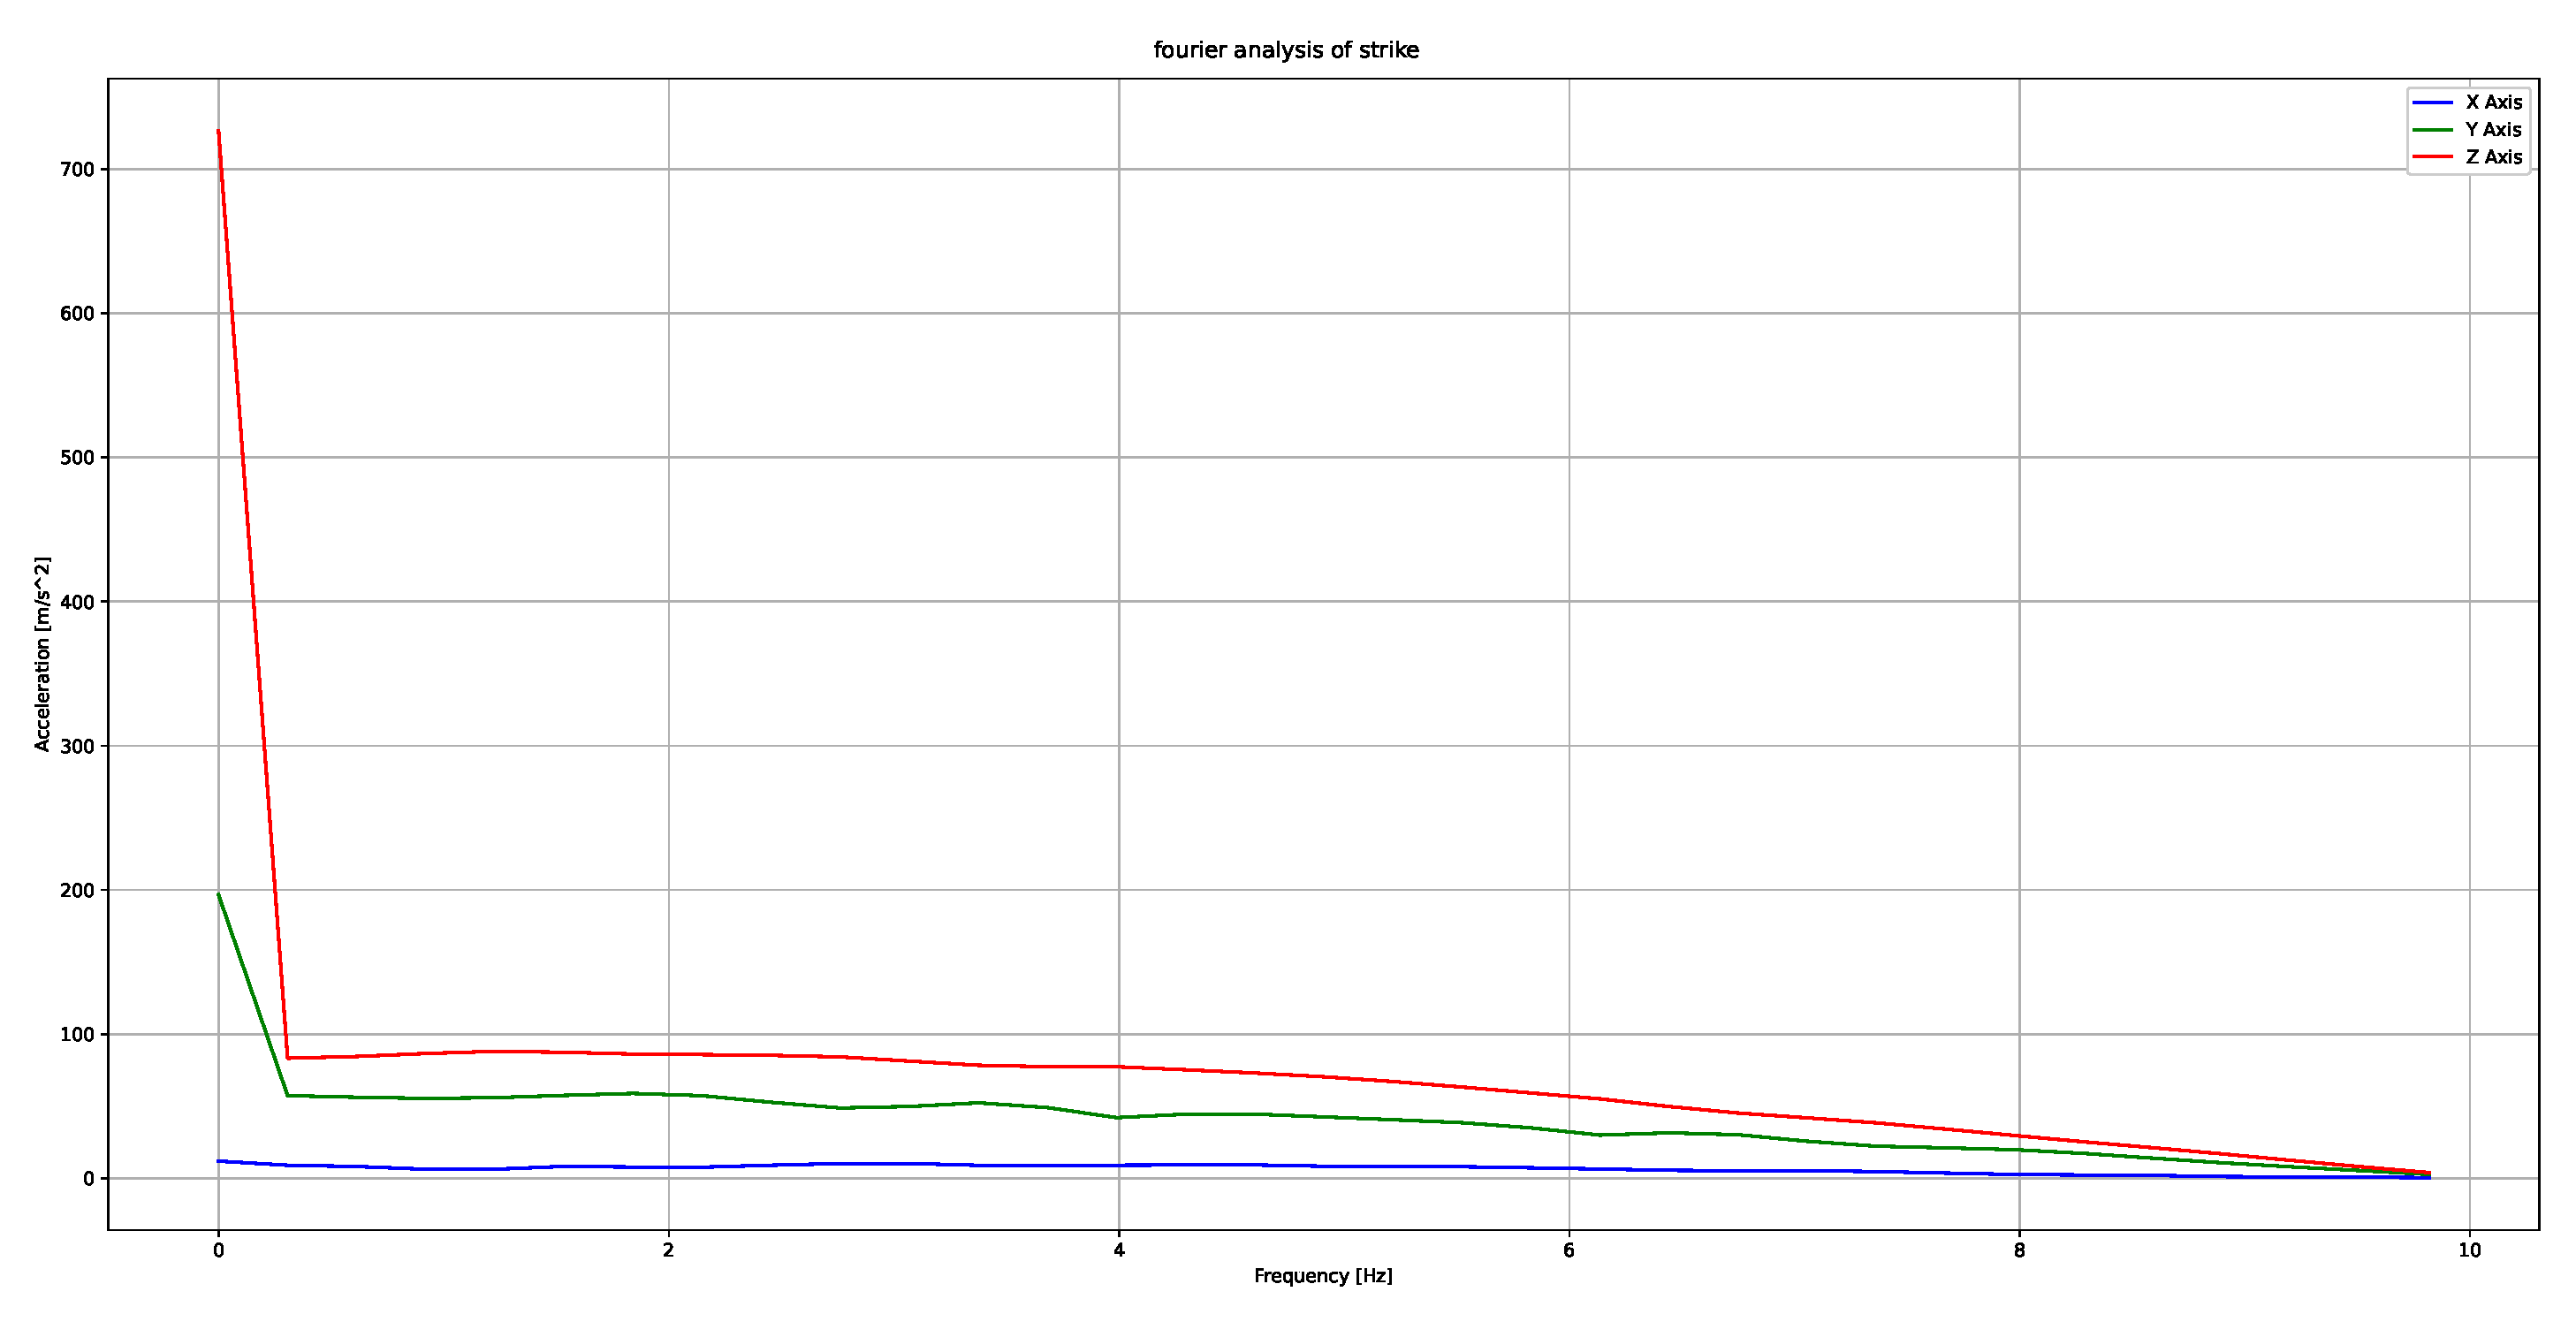
\includegraphics[width=0.8\textwidth]{resources/figures/Fourier_acceleration_strike.eps}
%     \caption{Fourier analysis of accelerometer data during the striking event}
%     \label{fig:fourier_accelerometer_striking}
% \end{figure}

% Looking at the Fourier transformed data no additional information could be extrapolated from the data, that wasn't already discussed from the untransformed data.

\vspace{30px}

\subsubsection{Dropping the MediColbox}

The accelerometer data, collected when the MediColbox was slowly and carefully
pushed off of a table, is presented in
Figure \ref{fig:accelerometer_dropping}.

here we observe the protope starts at rest with the
face of the \gls{hmi} facing directly upwards.
you then see a small time where an acceleration read is $0\;[m/s^2]$.
This is the time the protoype experiences free fall.
After the time of free fall we se a peak similar to the
impact during the striking with the dirrefence of the
read acceleration in $z$ direction goes from being positiveto being negative.
This change suggests that the prototype changes orientation from where the
face of the \gls{hmi} faces upwards to be facing downwards.

The maximum acceleration value recorded during the
drop was
$X = -7.7 [m/s^2]$, $Y = 35 [m/s^2]$, $Z = -50.7 [m/s^2]$,
which occurred at $t = 5.1[s]$.
The analysis confirms that the IMU effectively captured the
acceleration changes associated with the dropping event.

\begin{figure}[htbp]
    \centering
    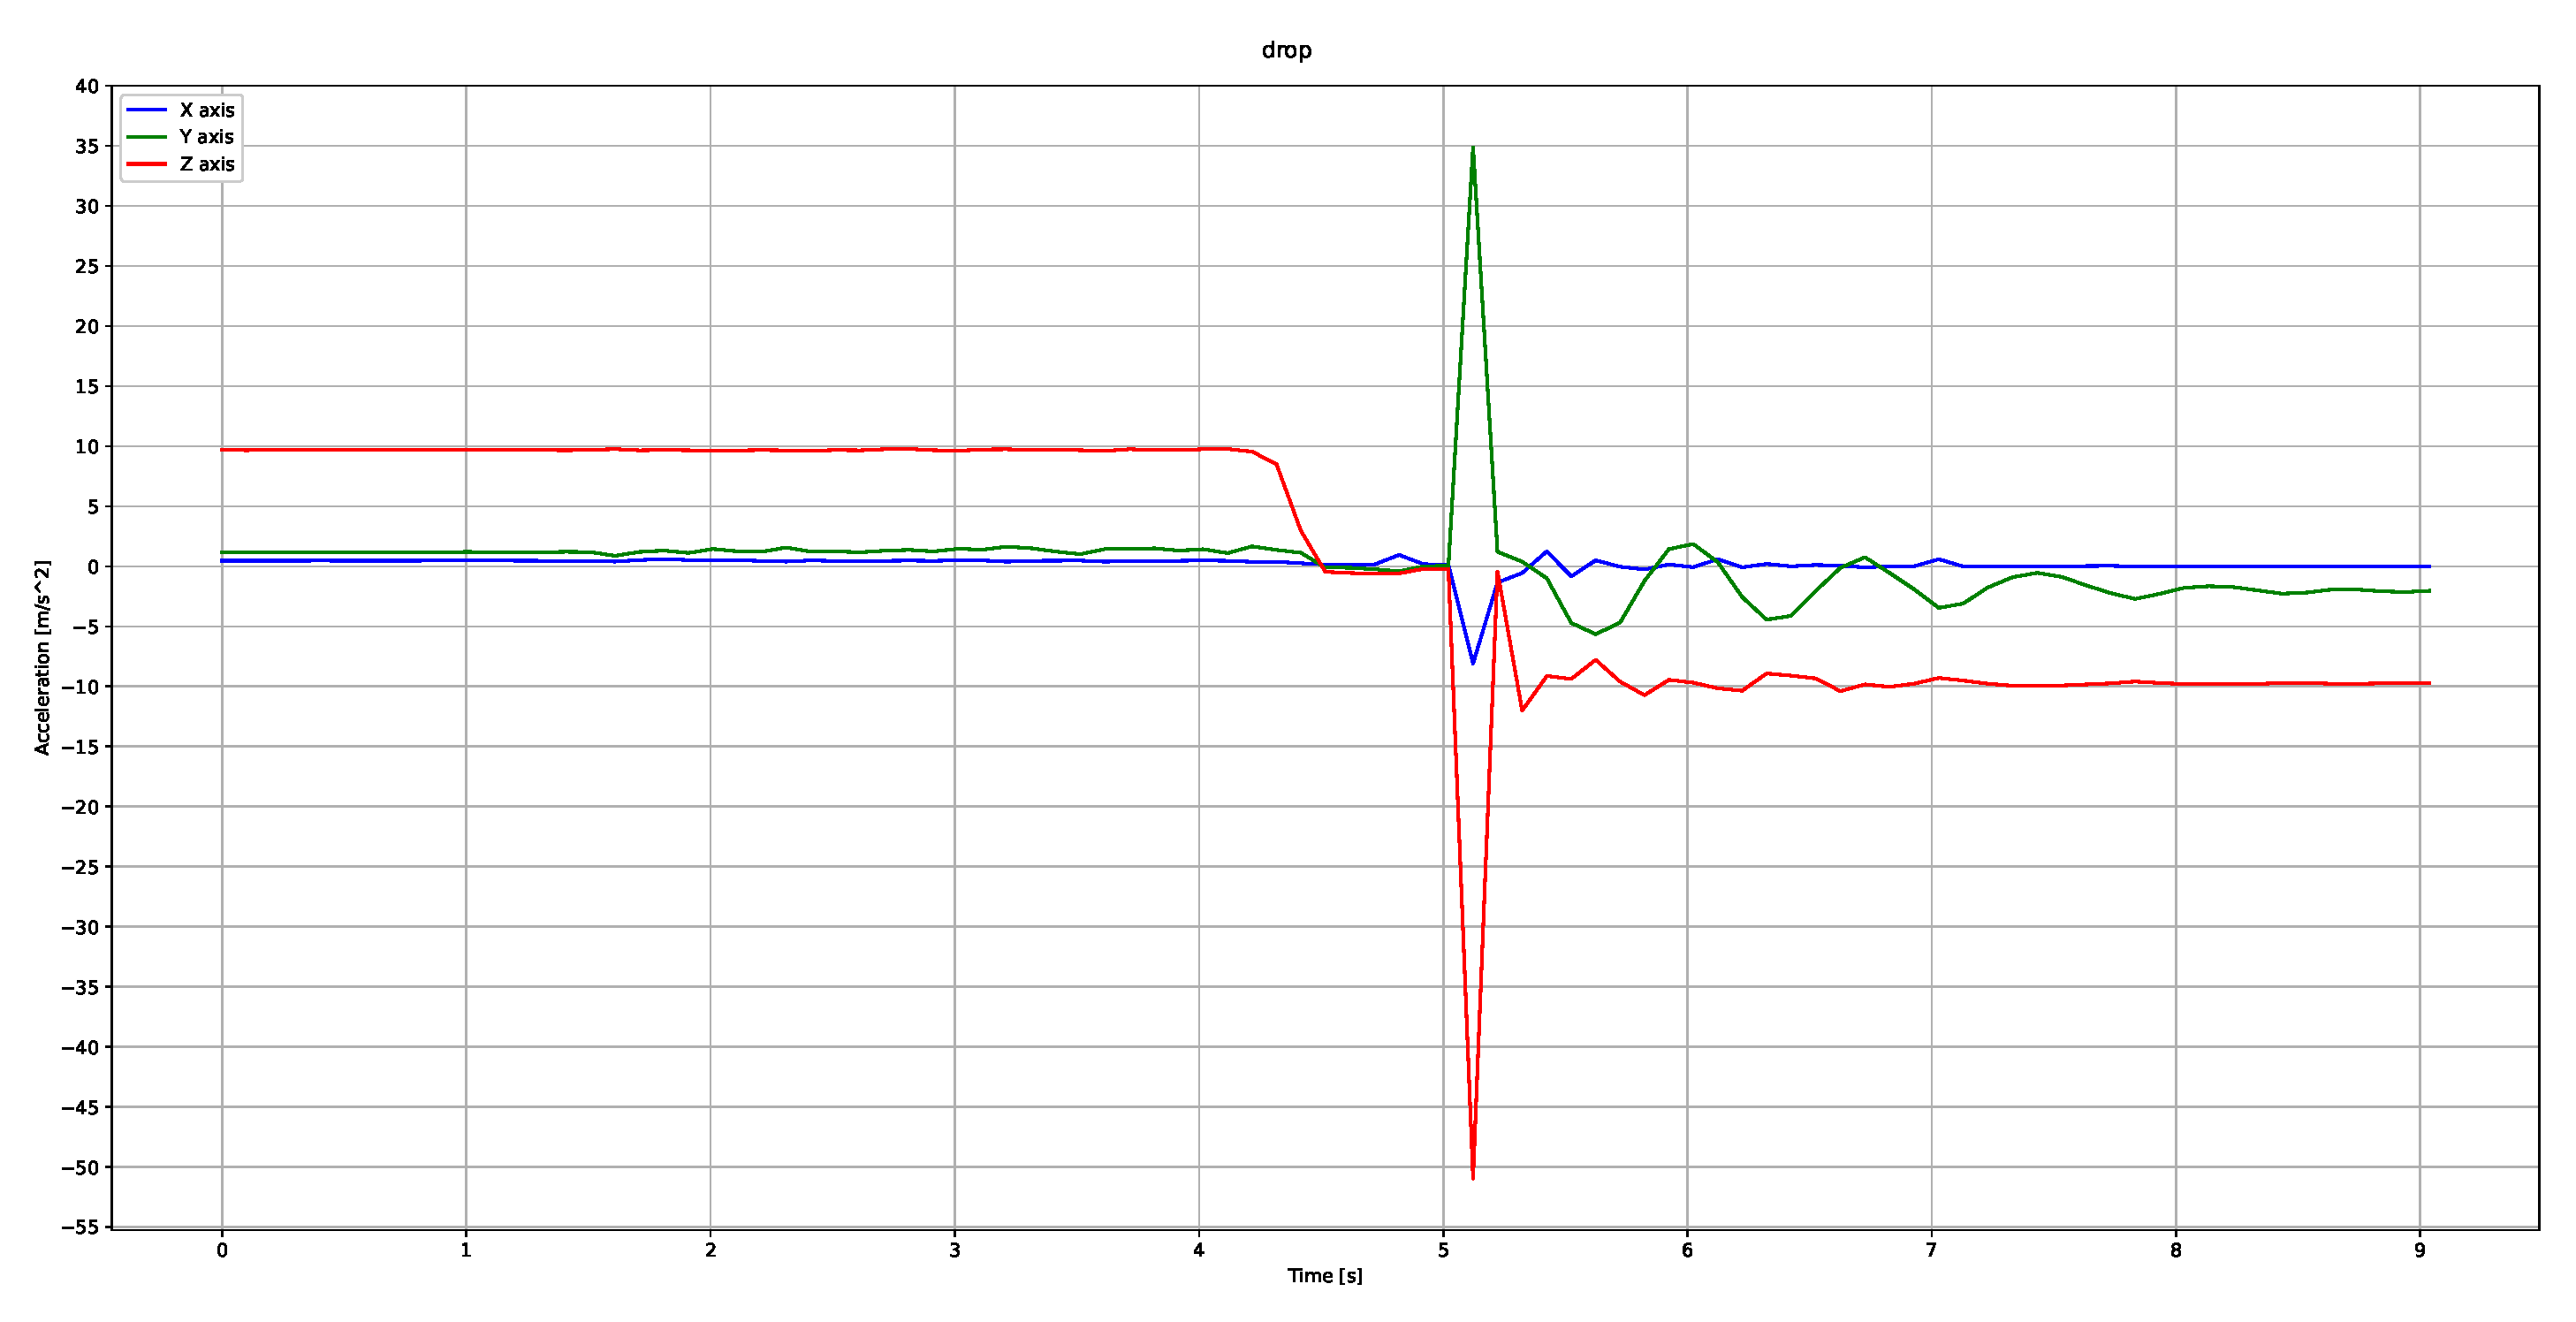
\includegraphics[width=0.8\textwidth]{resources/figures/Acceleration_drop.eps}
    \caption{Accelerometer data during the dropping event}
    \label{fig:accelerometer_dropping}
\end{figure}

Analyzing the data similarly to how we did at the striking event we find that in this case we have a total peak acceleration of $|\overrightarrow{a}| \approx 62 [m/s^2]$ this would already trigger the previously set trigger criteria of $60 [m/s^2]$. looking at the gyroscope data from Figure \ref{fig:gyroscope_dropping} we can see that there is also a lot of rotational movement starting as early as $t=4$ this suggests that the Prototype is rolling of the edge of where it was dropped from. this reading of roation confirms that the object was rotating when the acceleration suggested the prortype changed orientation.

\begin{figure}[htbp]
    \centering
    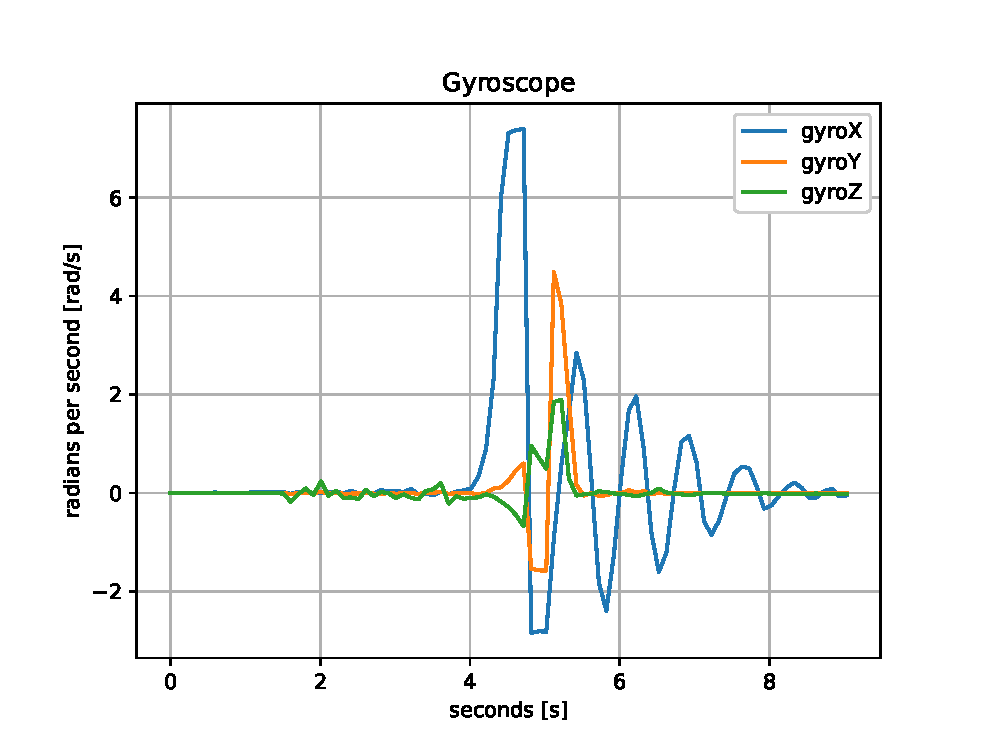
\includegraphics[width=0.8\textwidth]{resources/figures/Gyro_drop.eps}
    \caption{Gyroscope data during the dropping event}
    \label{fig:gyroscope_dropping}
\end{figure}

If we numerically integrate the Gyroscope's angular velocity over time to make position we get an estimate of pose visualized in Figure \ref{fig:pose_dropping}.

we can approximate this by multiplying the time difference $\Delta t$ at any point $i$ of reading, with the meassured angular velocity $\frac{d \theta}{dt}$ from the gyroscope at that same point $i$, and accumulate it over time, making the current accumulated changes in angle of time at the point $i$ to be the current angle $\theta$ at that point $i$.

$$\int \frac{d \theta}{dt} dt \approx \sum_{i=0} \frac{d {\theta}_{i}}{dt} {\Delta t}_{i} = {\theta}_{i} $$


\begin{figure}[htbp]
    \centering
    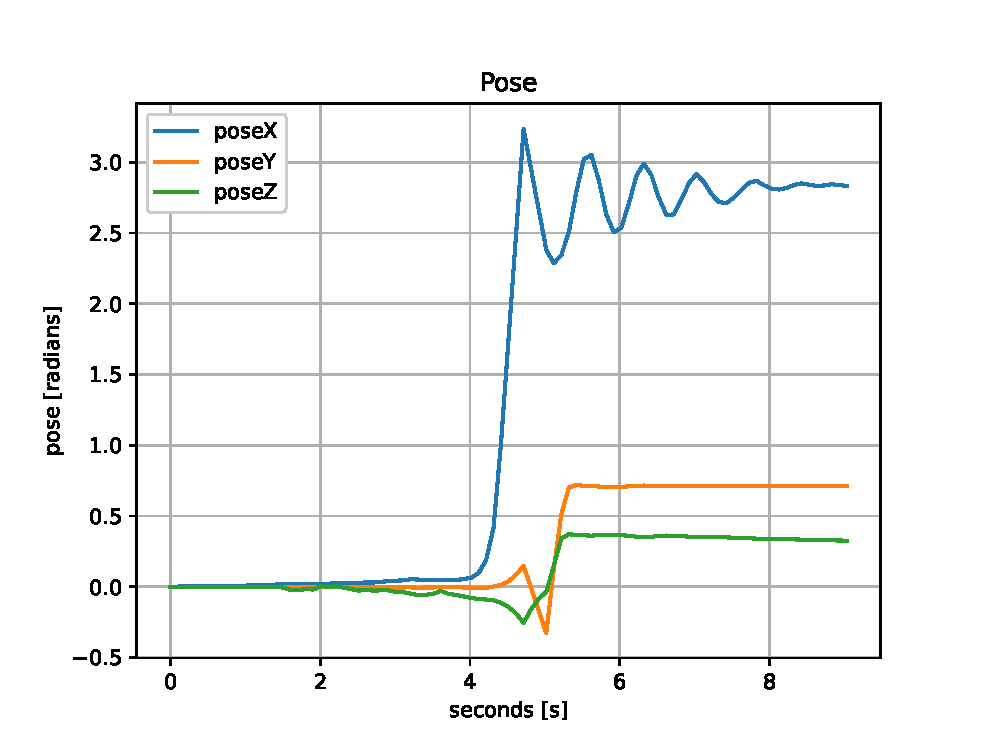
\includegraphics[width=0.8\textwidth]{resources/figures/Pose_drop.eps}
    \caption{Pose estimate during the dropping event}
    \label{fig:pose_dropping}
\end{figure}

In the pose data we notice that the estimated pose changes by approximately $3.1 [rad]$ (about $180$ degrees) in between time $t=4$ and $t=4.7$ this strongly suggest that the Protoype has roled half a round around the $X$-axis. This is supported in how the acceleration (Figure \ref{fig:accelerometer_dropping}) shows the $Z$-axis changes from being positive to being negative.
The pose changing in such drastic ways will be representative of how a box can be tipped over or turned around during an intrusion attempts when an intruder tries to figure out where to attack. Integrating position and velocity from acceleration and pose is also possible and combining the accumulated change in pose and the accumulated change in change of position might be valuable when the box wants to detect if somebody picks up the box and/or moves it to somewhere it shouldn't be. Using this we could theoretically set an area of where box is restricted to be within or outside.

A problem with this is that differentiating between intrusion attempts and just any random regular use is near impossible, and combined with how accumulating values also result in accumulated error. This makes any estimate less accurate over time, and reliability-maximizing algorithms, will be necessary if we are to do anything over longer time with this data with accumulating error.

However, even though the gyroscope data alone cannot help without increasing reliability, we can by using newtons first law (a body at rest experiences a sum of zero forces in any direction) make use of the orientation of the read normal force at every time when the magnitude is close to the local gravitational constant.

$$\sum F = m \sum a = 0$$

$$\sum F = F_{normal} + F_{gravity} = 0$$

Using this logic we can say that if $a=0$ then $F_{normal} + F_{gravity} = 0$ meaning that $|F_{normal}| = |F_{gravity}|$ and the two vectors points opposite to each others.

this way we can estimate the orientation of the prortype using the accelerometer. and an algorithm saying that any time we detects the protoype being tipped on the side, or up side down, should be a time where we should sound the alarm.

giving us an aditional trigger to the alarm triggering algorithm.

If the angle of the prototype in pith and/or roll, changes to become equal to, or greater than $90$ degrees plus minus an error value, then trigger the alarm.

% Moving on to the Fourier analysis of the accelerometer data during the
% dropping event (Figure \ref{fig:fourier_accelerometer_dropping}.)
% Here there is again little information to gain.

% \begin{figure}[htbp]
%     \centering
%     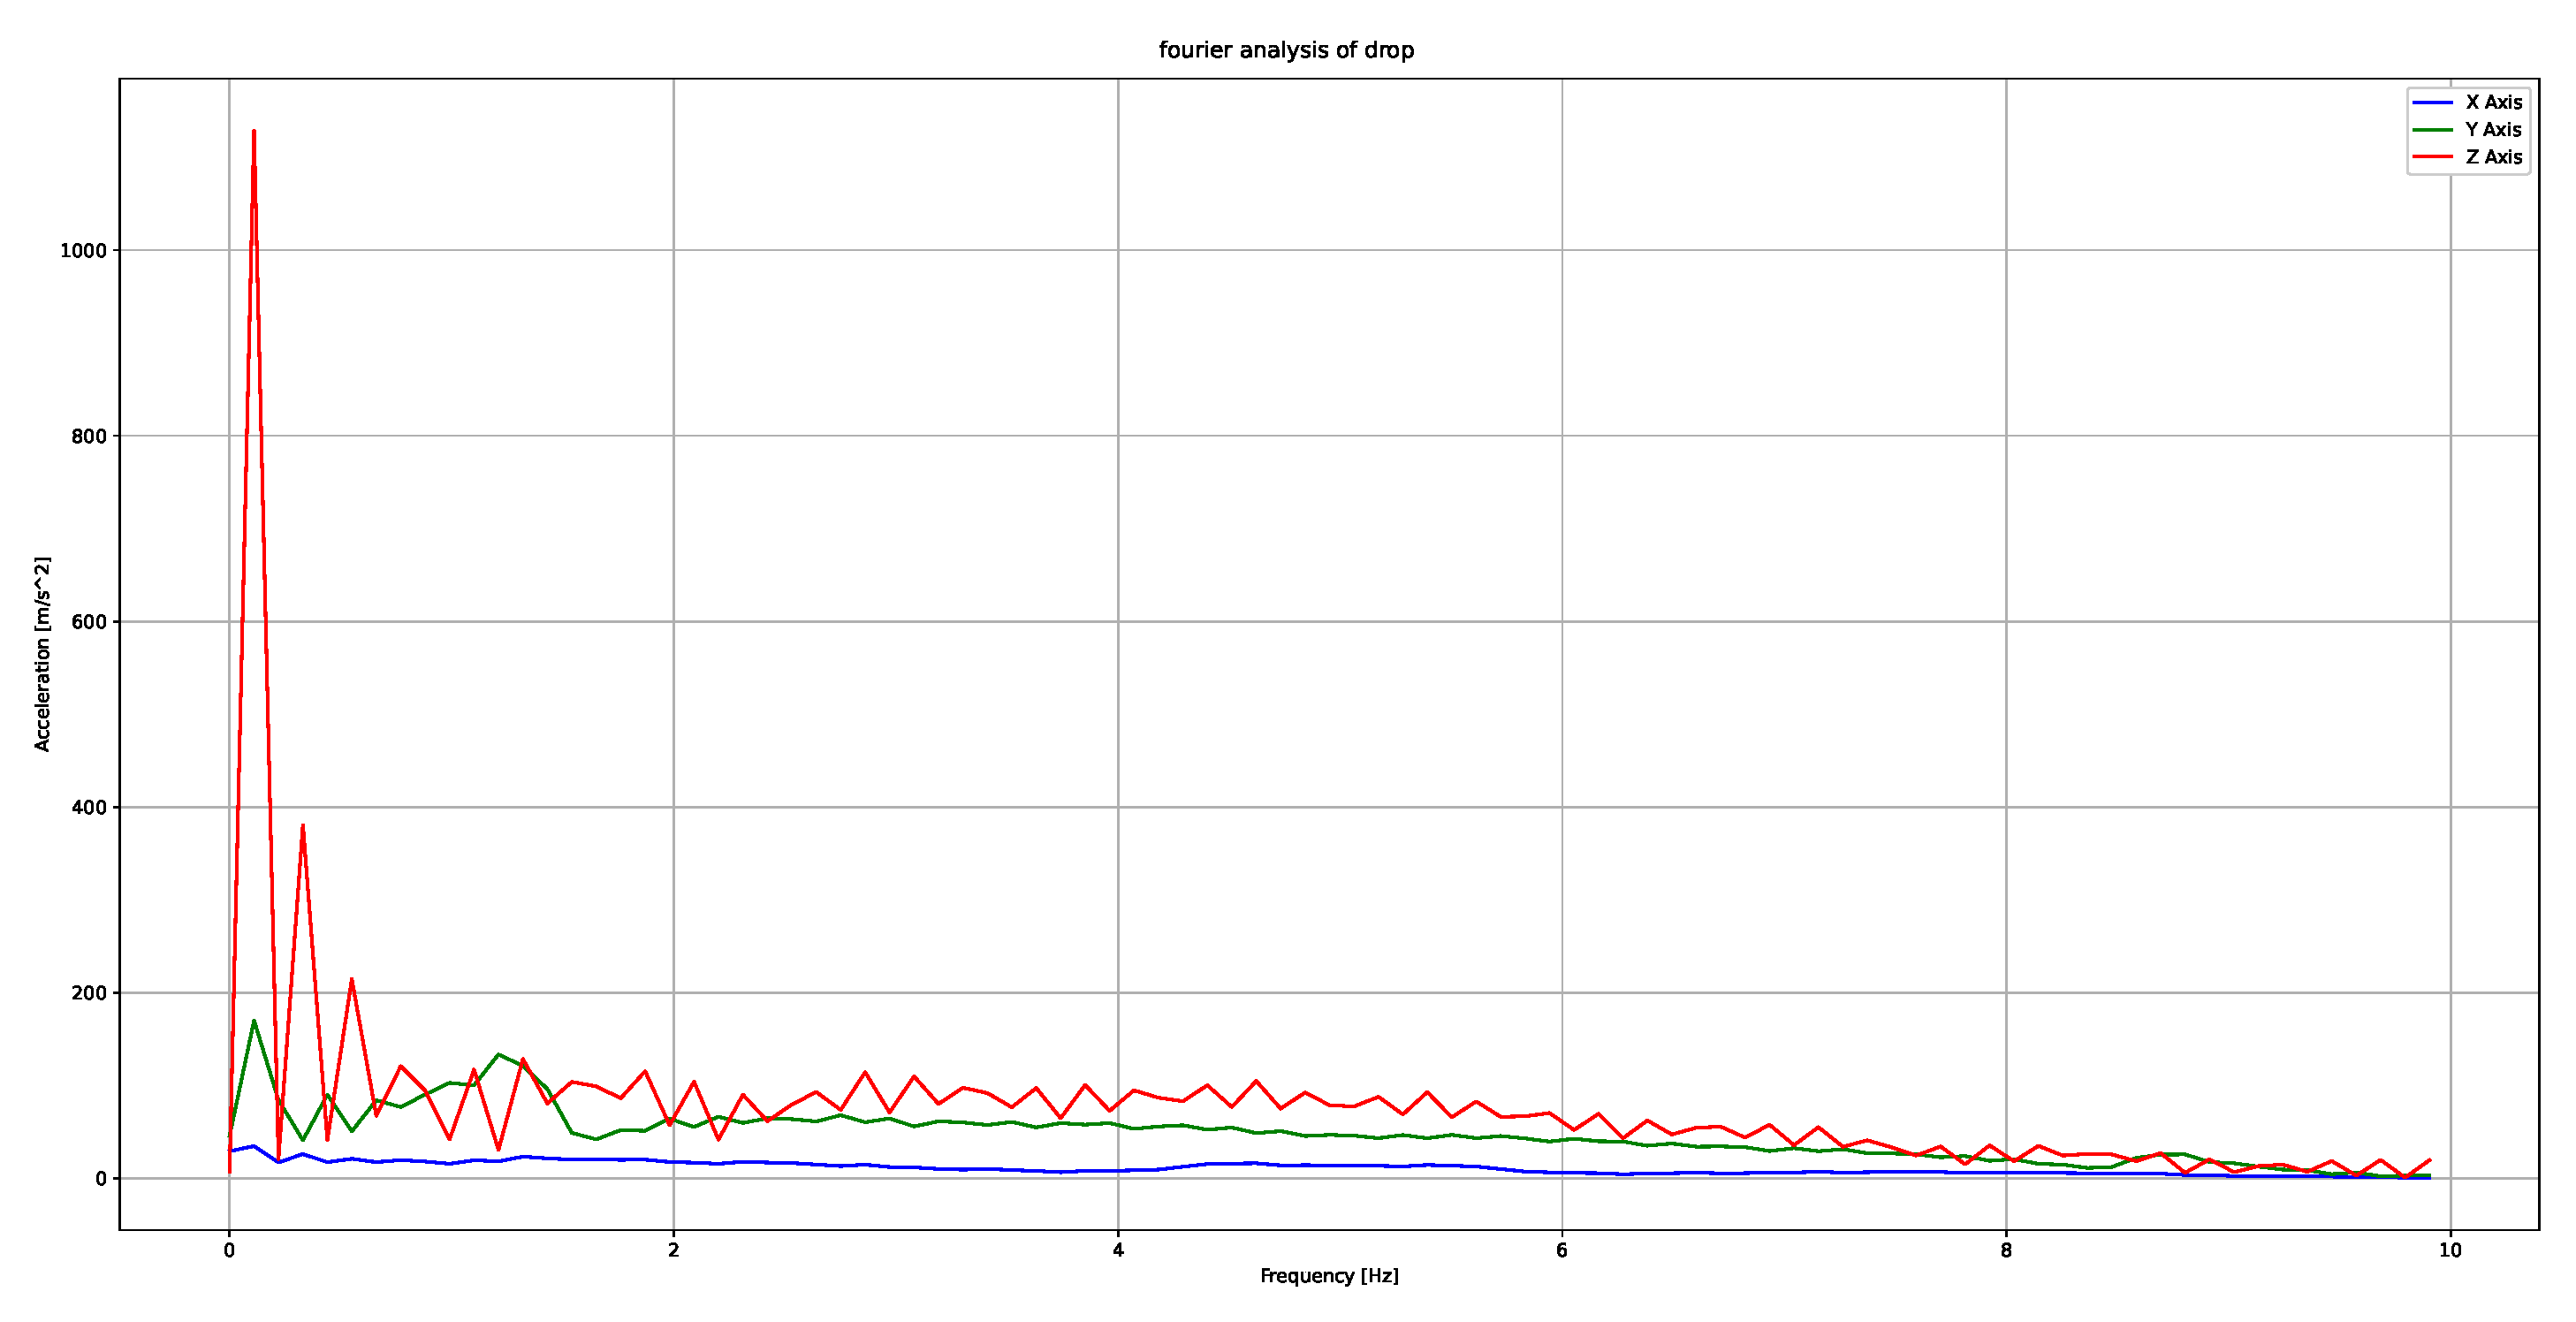
\includegraphics[width=0.8\textwidth]{resources/figures/Fourier_acceleration_drop.eps}
%     \caption{Fourier analysis of accelerometer data during the dropping event}
%     \label{fig:fourier_accelerometer_dropping}
% \end{figure}

\vspace{30px}

\subsubsection{Sawing on the MediColbox}

This event is tested by mounting the prototype to a wooden plank, and sawing in that plank using a hacksaw.

Figure \ref{fig:accelerometer_sawing} illustrates the
accelerometer data recorded while sawing on the
MediColbox using a metal cutting saw.
The data exhibited periodic variations in acceleration
corresponding to the back-and-forth sawing motion.
The analysis of the data indicated a consistent pattern of
acceleration changes during the sawing event. This suggests that the IMU was able to capture the vibrations and oscillations caused by the sawing action.

\begin{figure}[htbp]
    \centering
    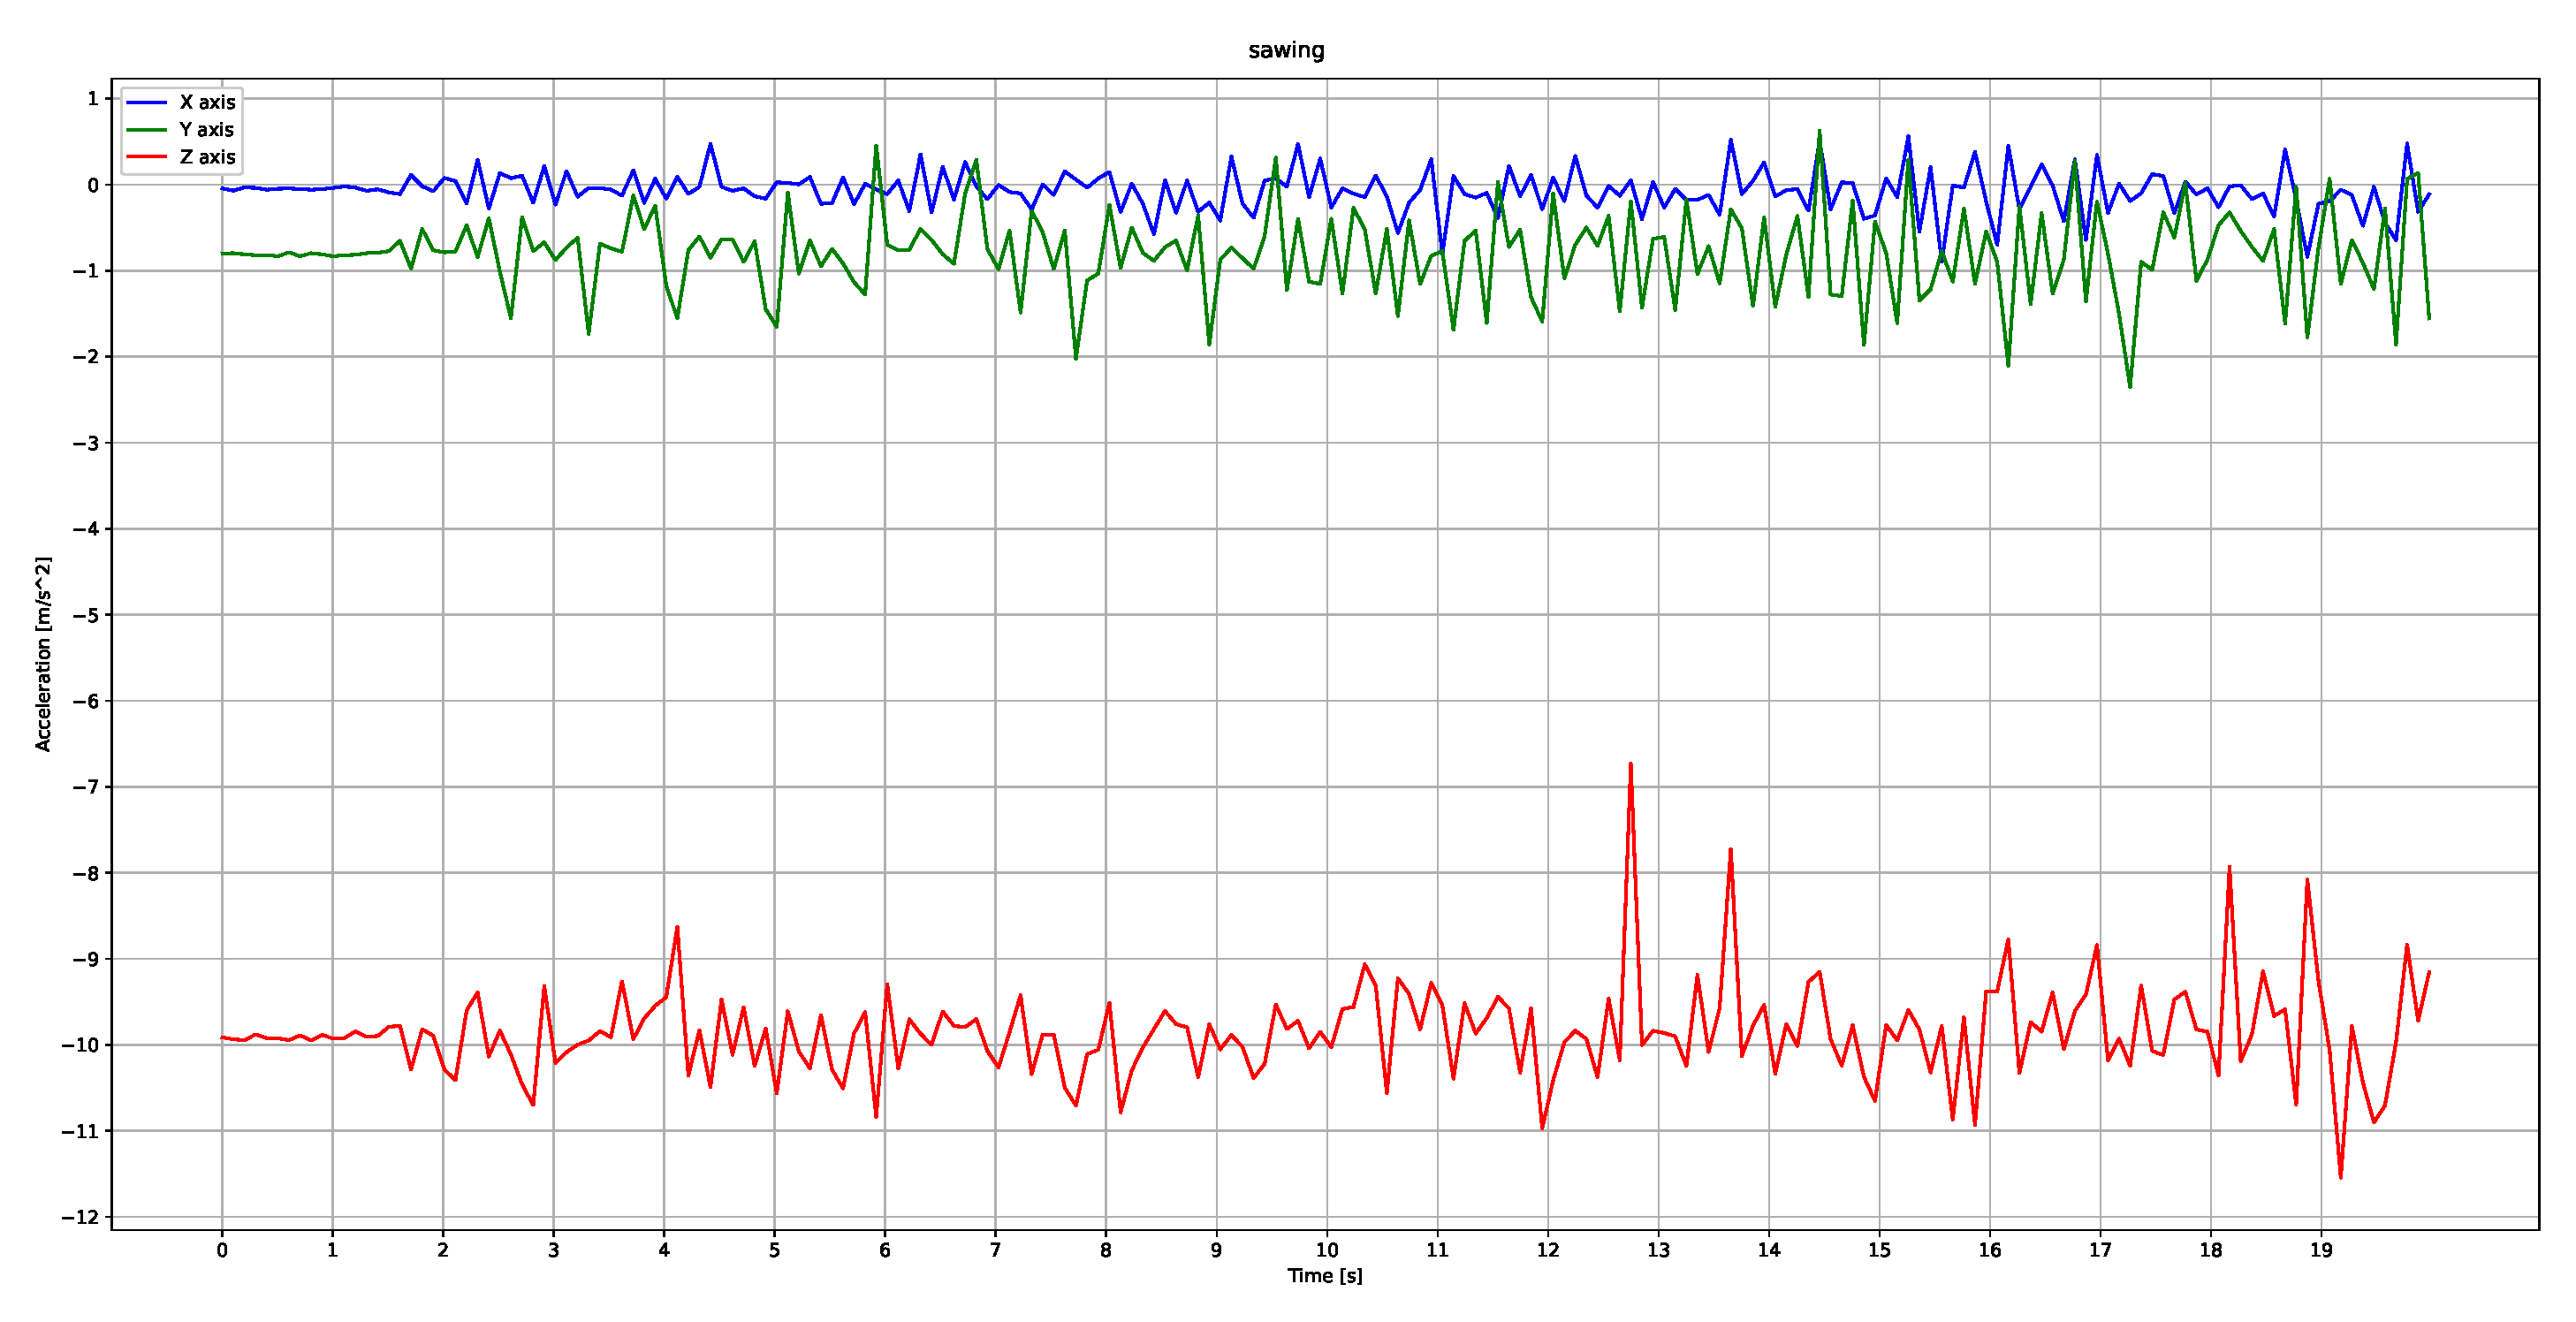
\includegraphics[width=0.8\textwidth]{resources/figures/Acceleration_sawing.eps}
    \caption{Accelerometer data during the sawing event}
    \label{fig:accelerometer_sawing}
\end{figure}

The Fourier analysis of the accelerometer data during the sawing event is shown in Figure \ref{fig:fourier_accelerometer_sawing}. The Fourier analysis allows us to examine the frequency components present in the accelerometer readings and provides insights into the characteristics of the sawing action. By analyzing the frequency distribution and identifying prominent peaks or patterns in the frequency domain, we can gain a deeper understanding of the dynamic response of the MediColbox to the sawing forces.

\begin{figure}[htbp]
    \centering
    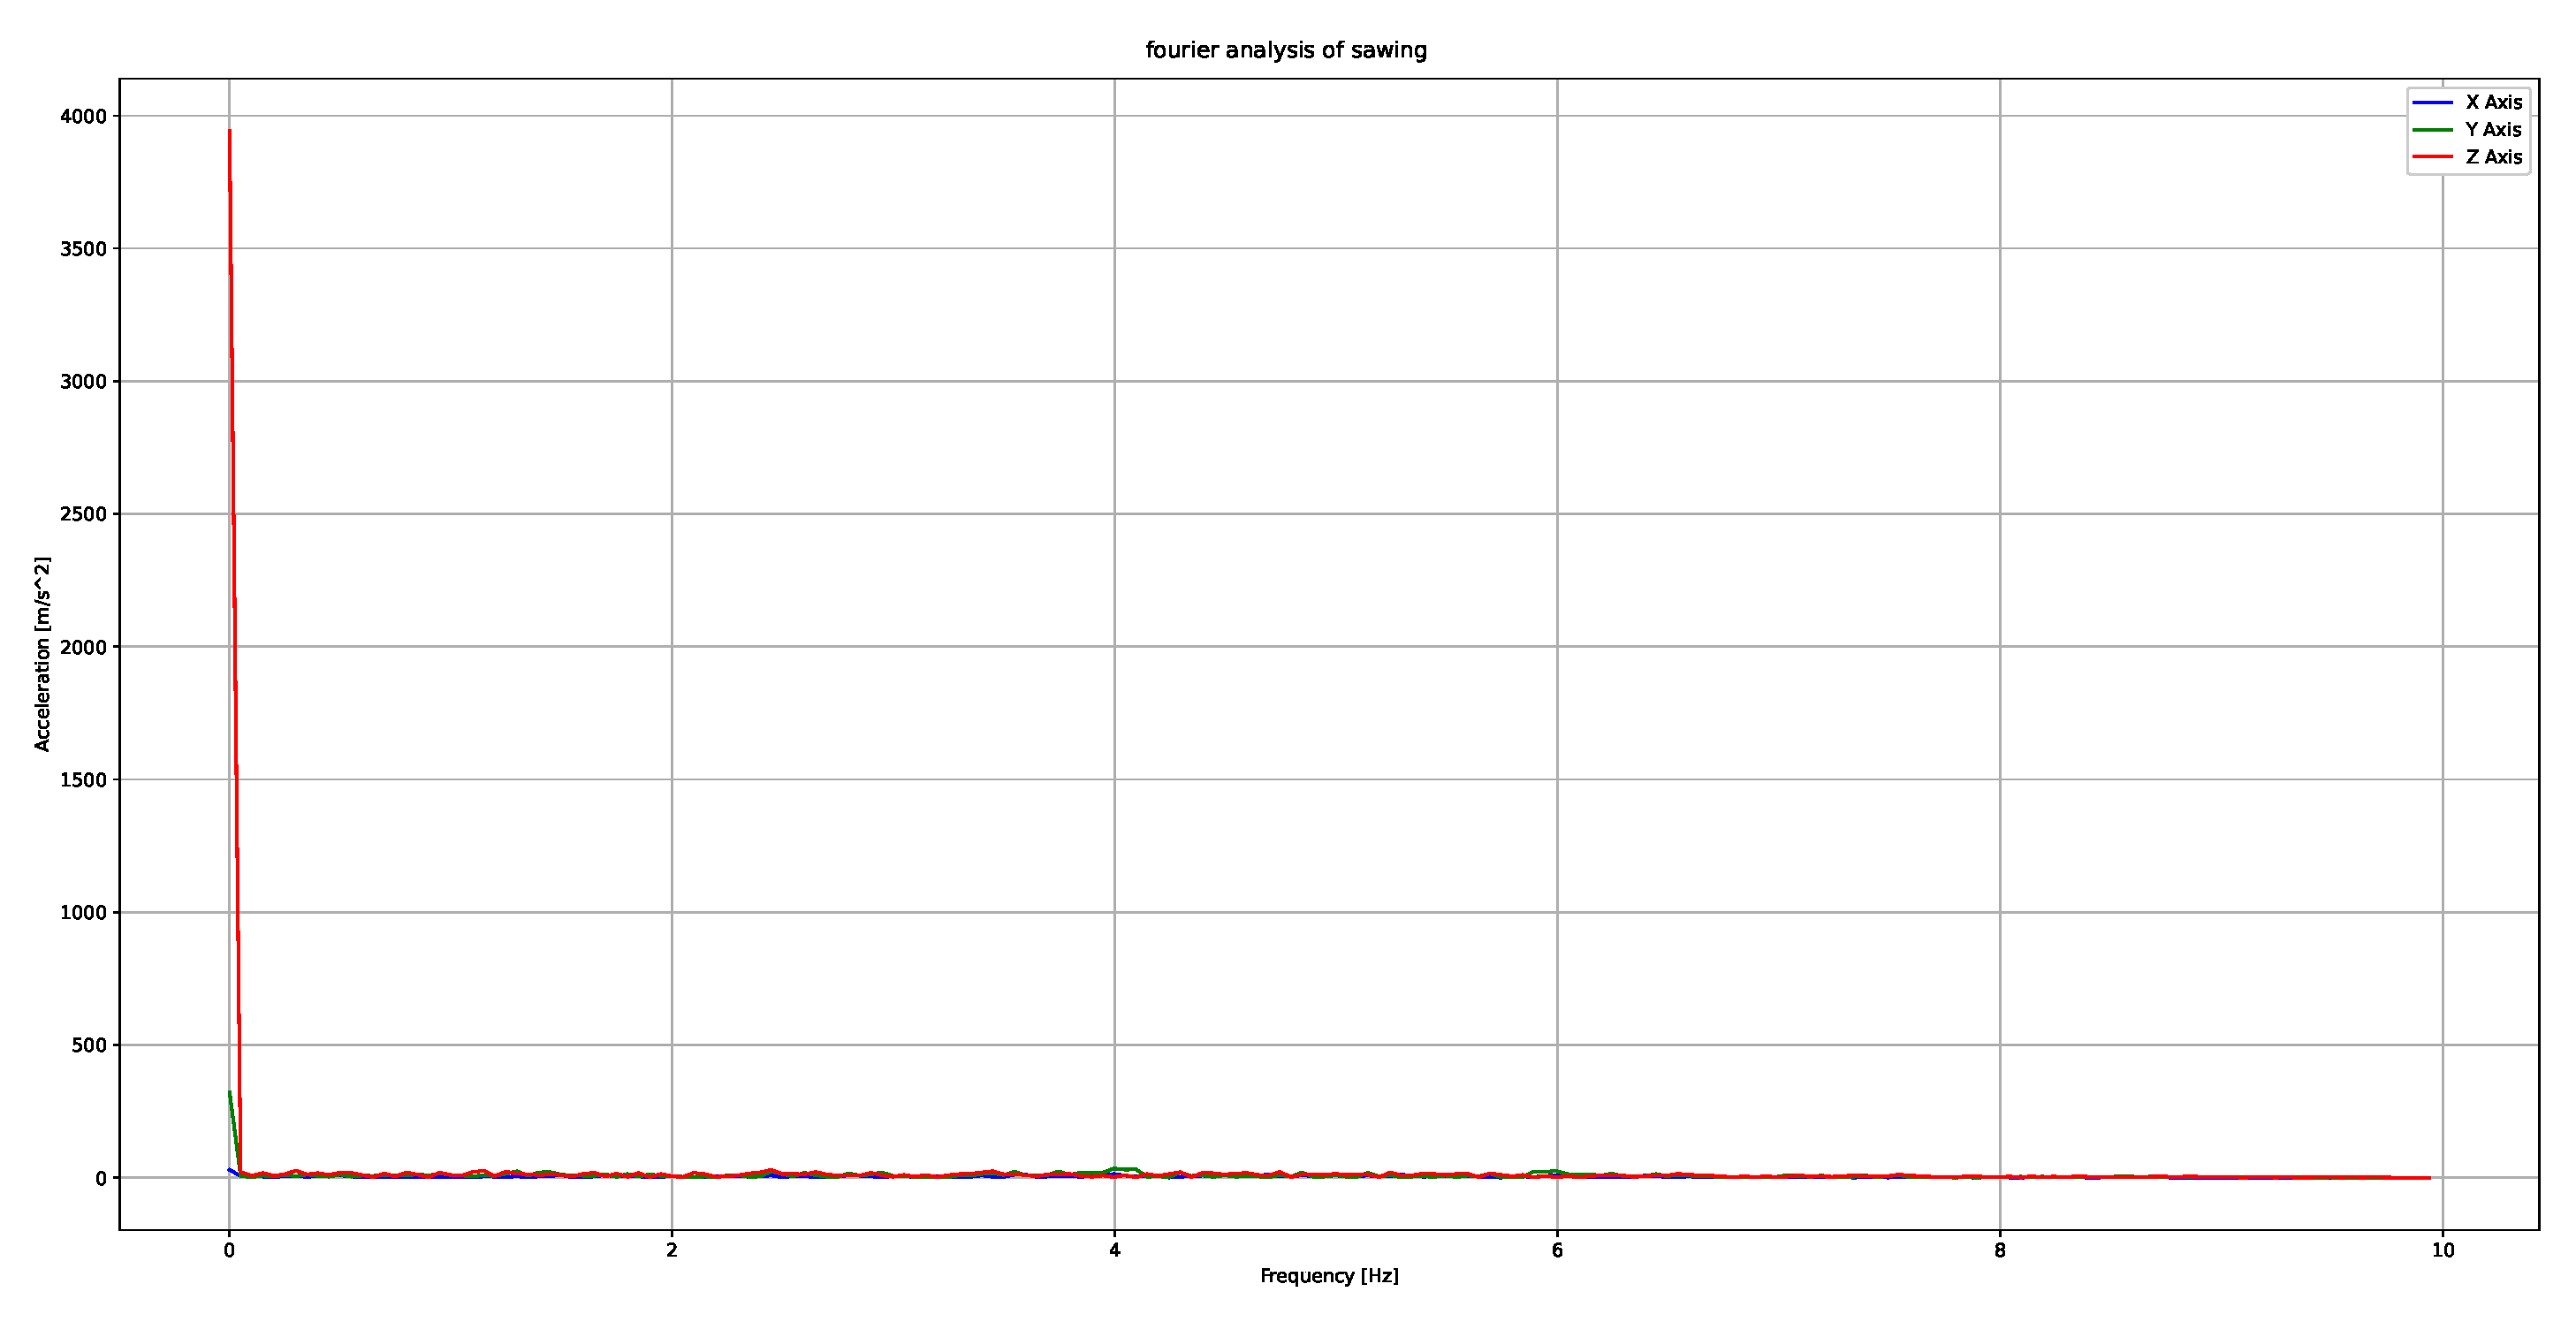
\includegraphics[width=0.8\textwidth]{resources/figures/Fourier_acceleration_sawing.eps}
    \caption{Fourier analysis of accelerometer data during the sawing event}
    \label{fig:fourier_accelerometer_sawing}
\end{figure}

\clearpage

\subsubsection{Shaking the MediColbox}

The accelerometer data obtained while shaking the
MediColbox on a sifter,
simulating cutting it with an angle grinder,
is presented in Figure \ref{fig:accelerometer_shaking}.
The data exhibited irregular and rapid fluctuations in
acceleration due to the shaking motion.
The analysis of the data demonstrated that the IMU was
sensitive enough to detect and record these rapid changes in
acceleration, indicating its potential for
detecting unauthorized access attempts involving
similar movements.

\begin{figure}[htbp]
    \centering
    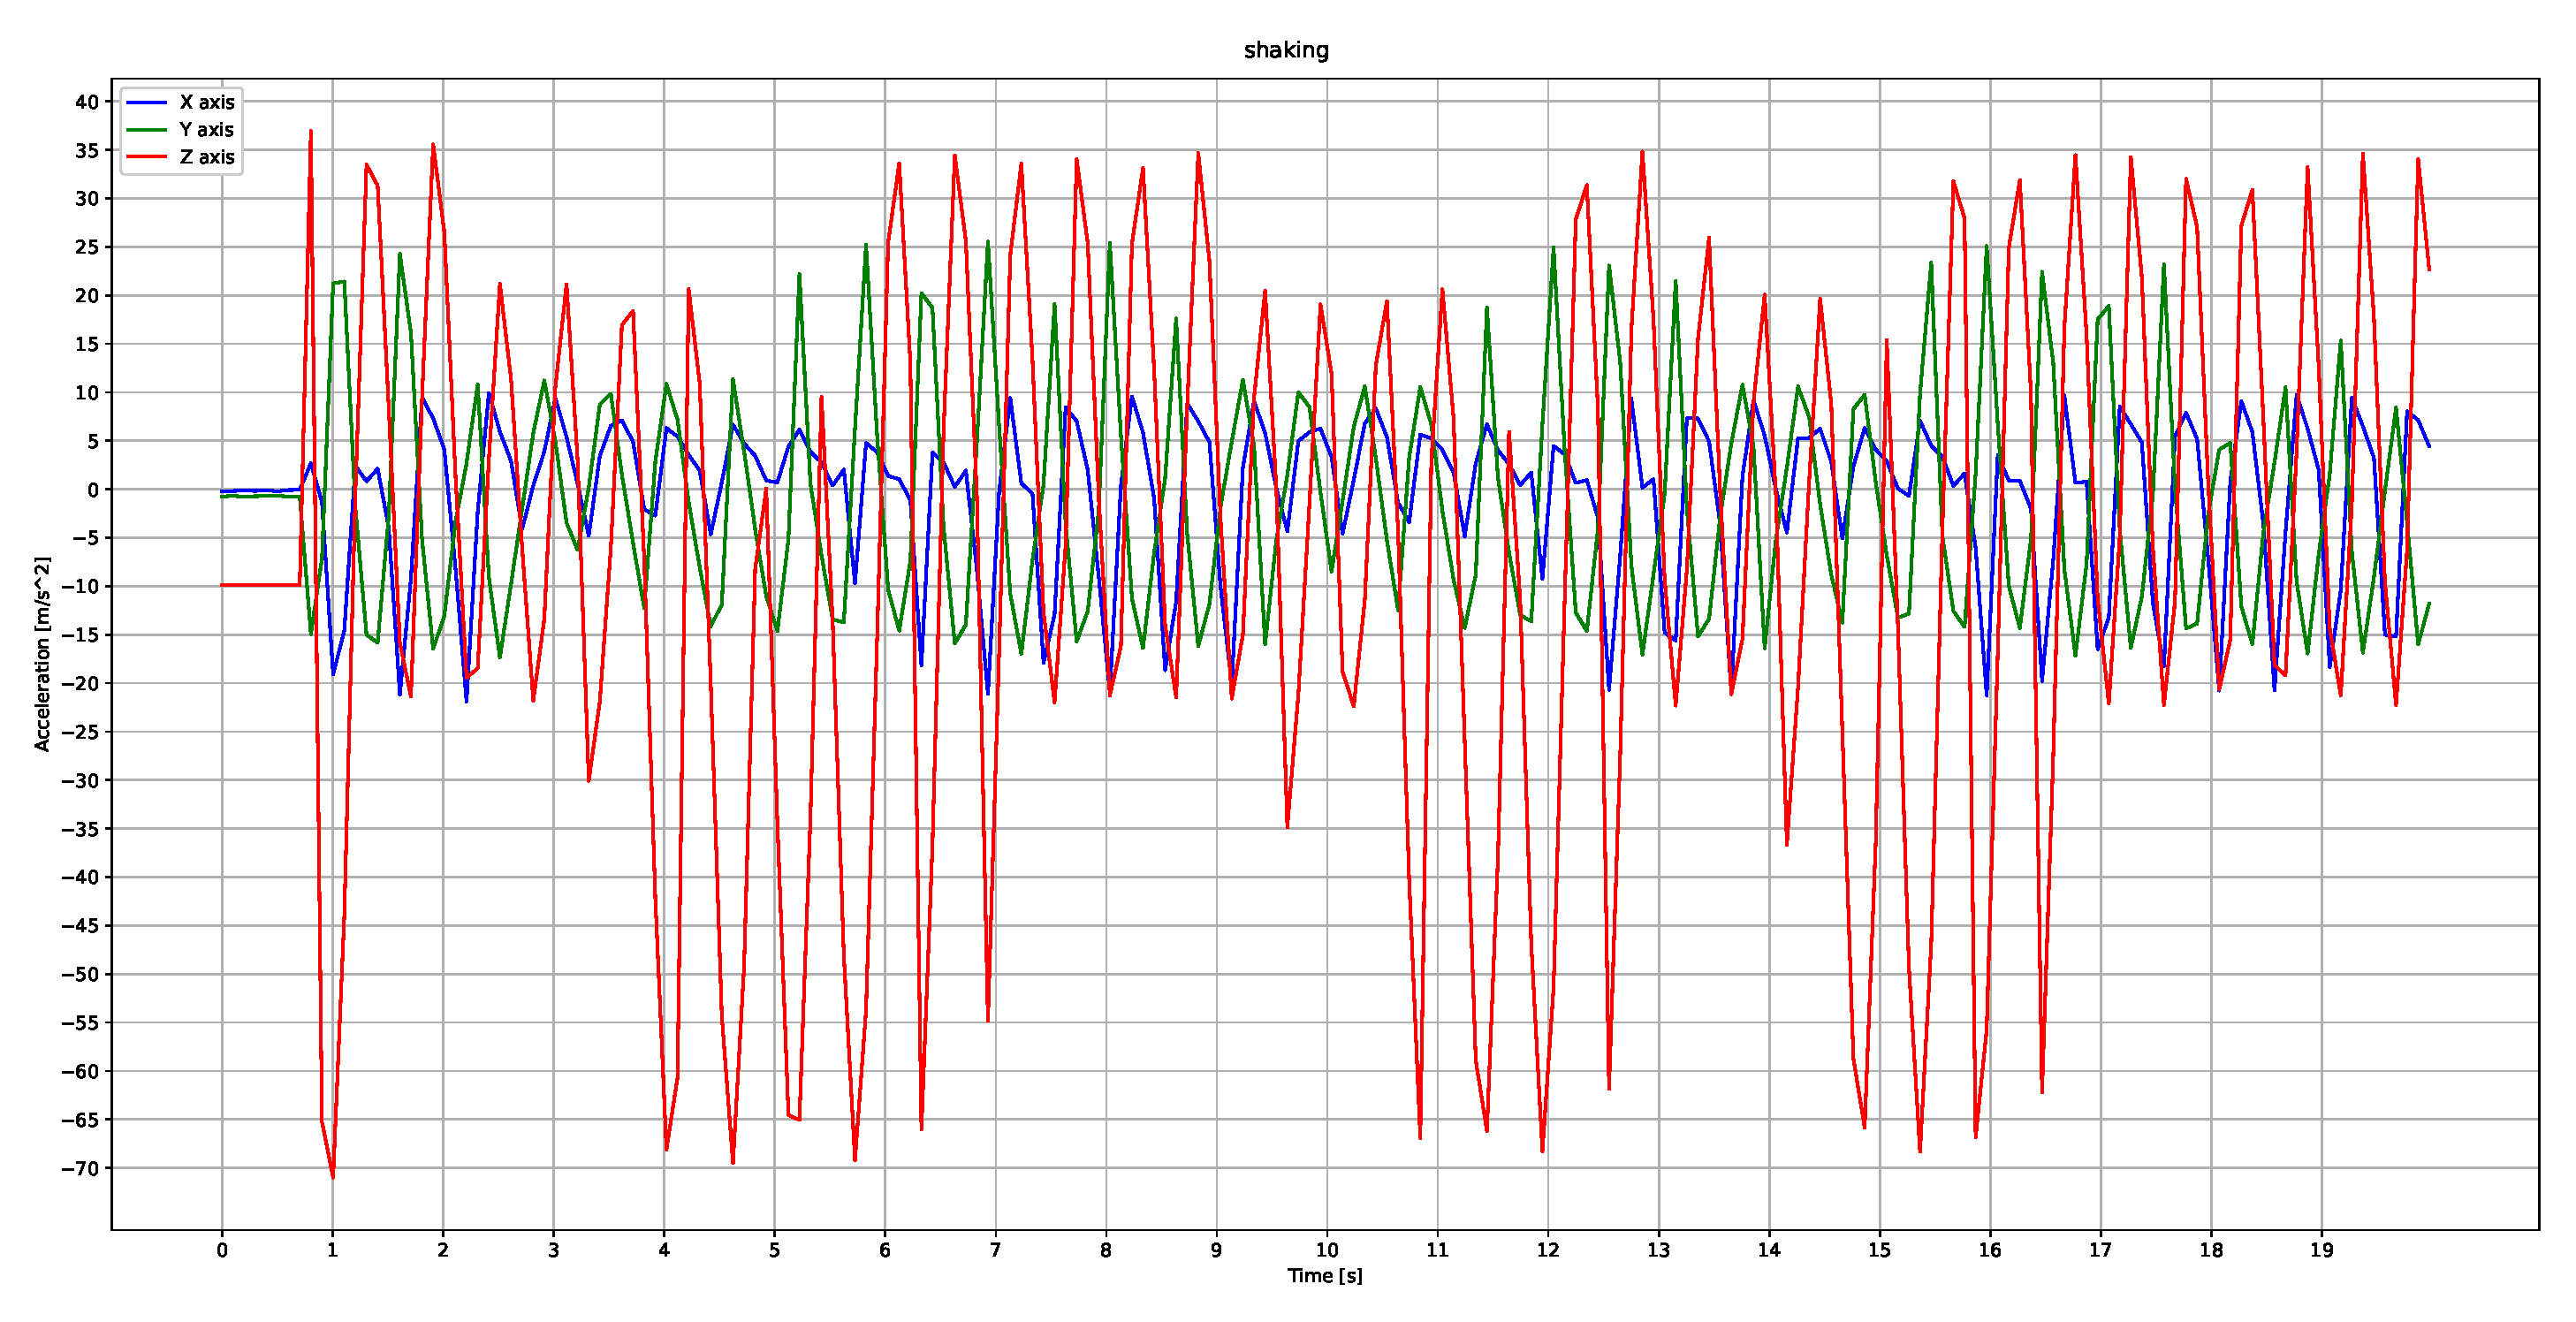
\includegraphics[width=0.8\textwidth]{resources/figures/Acceleration_shaking.eps}
    \caption{Accelerometer data during the shaking event}
    \label{fig:accelerometer_shaking}
\end{figure}

The Fourier analysis of the accelerometer data during the
shaking event is shown in
Figure \ref{fig:fourier_accelerometer_shaking}.
The Fourier analysis allows us to examine the
frequency components present in the accelerometer readings and
provides insights into the characteristics of the shaking motion.
By analyzing the frequency distribution and
identifying prominent peaks or patterns in the frequency domain,
we can gain a deeper understanding of the
dynamic response of the MediColbox to the shaking forces.


\begin{figure}[htbp]
    \centering
    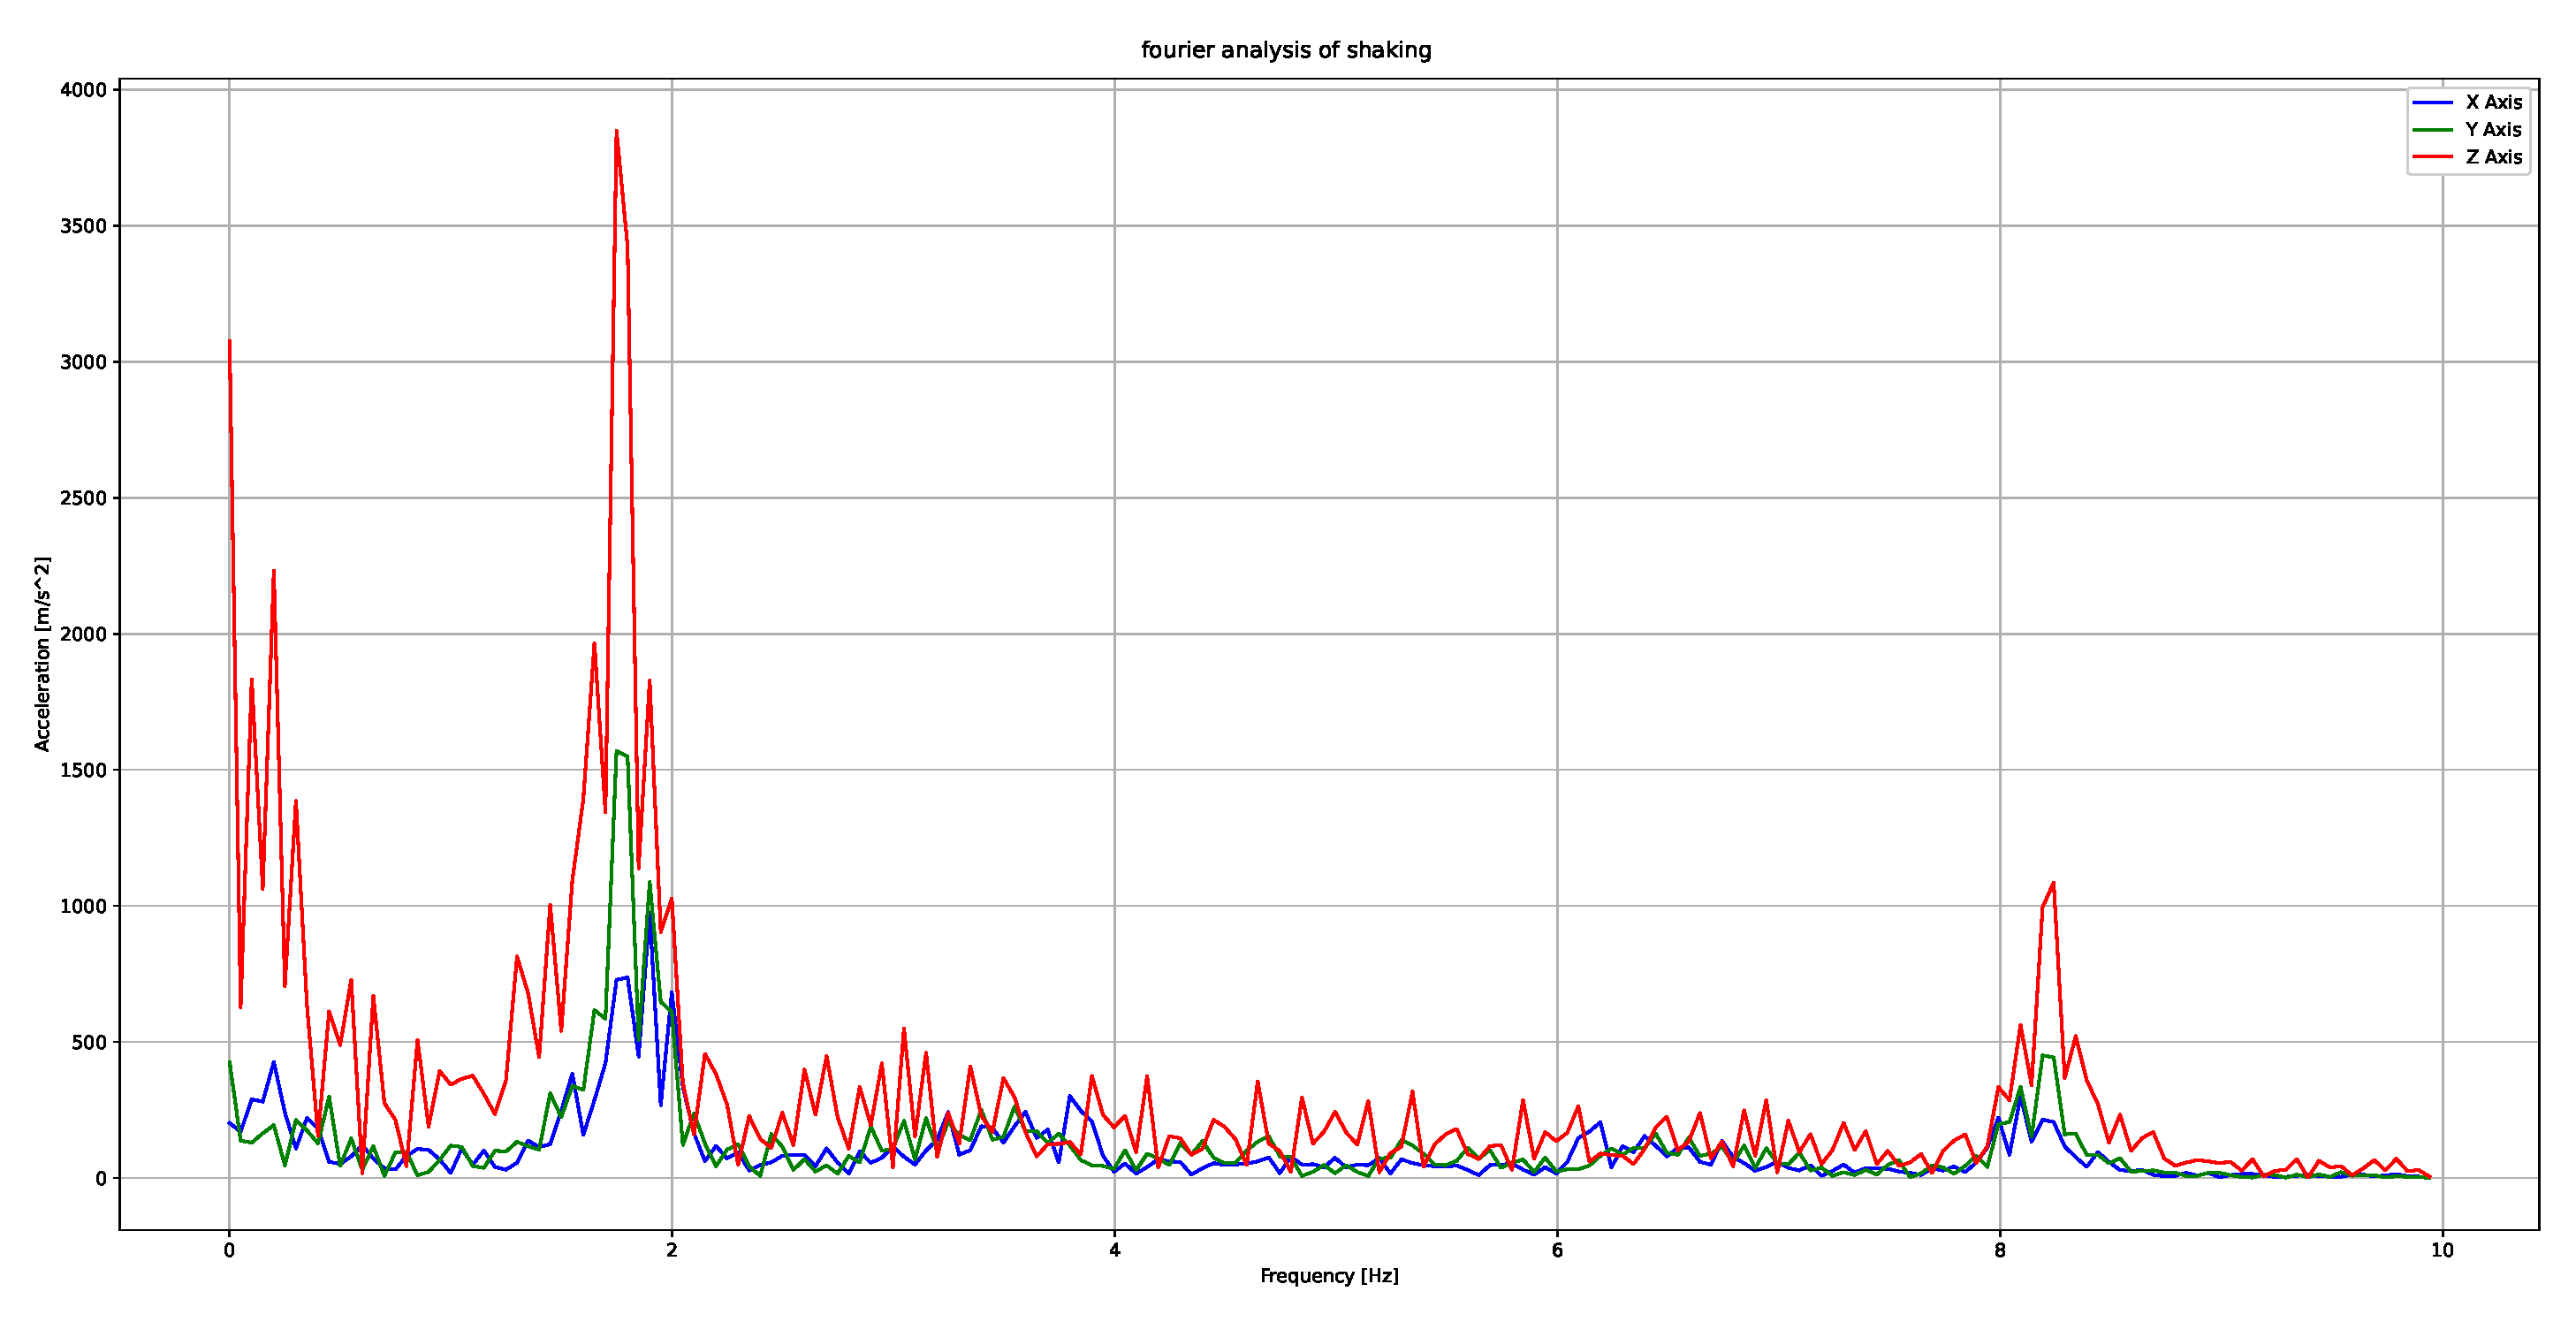
\includegraphics[width=0.8\textwidth]{resources/figures/Fourier_acceleration_shaking.eps}
    \caption{Fourier analysis of accelerometer data during the shaking event}
    \label{fig:fourier_accelerometer_shaking}
\end{figure}

\subsection{Discussion of Findings}

The analysis of the accelerometer data during the
simulated intrusion attempts provides valuable insights into the
IMU's ability to detect and capture unauthorized access events.
The results demonstrate that the
accelerometer readings accurately captured the
accelerative patterns associated with striking,
dropping, sawing, and shaking the MediColbox.

The findings suggest that the IMU is a reliable and
effective sensor for detecting physical movements and vibrations,
which are indicative of intrusion attempts.
The accelerometer data recorded during the
simulated scenarios showcased the IMU's sensitivity to
changes in acceleration,
enabling it to capture both high-impact events and
subtle vibrations.

However, it is important to note that the analysis
focused solely on the accelerometer data,
and other data collected by the IMU,
such as gyroscope or magnetometer readings,
were not considered in this study.
Further research could explore the
integration of multiple sensor data to enhance the
accuracy and robustness of intrusion detection.

Overall, the results indicate the potential of the IMU as
a standalone solution for intrusion detection on the
MediColbox. The findings support the feasibility of
utilizing the IMU to enhance the security and protection of the
MediColbox by effectively detecting and alerting on
unauthorized access attempts.

\end{document}